\chapter{Notions de calcul vectoriel}
\label{sec:calcvec}

Chapitre en construction!

%%%%%%%%%%%%%%%%%%%%%%%%%%%%%%%%%%%%%%%%%%%%%%%%%%%%%%%%%%%%%%%%%%%%%%
\section{Les Vecteurs}
\label{sec:vec}

Un vecteur-géométrique est une quantité physique représentée par \textbf{une amplitude et une direction}. Lorsqu'une base vectorielle est spécifiée, un vecteur peut alors être représenté par des composantes scalaires selon chaque vecteur unitaire de la base. Il est important de distinguer la notion de vecteur-géométrique $\vec{v}$ et de ses composantes regroupées dans un vecteur colonne $\col{v}$, surtout lorsque plusieurs bases sont utilisés. 

La notation suivant est utilisée dans ces notes:
%%%%%%%%%%%%%%%%%%%%%%%%%%%%%%%%%%%
\begin{align}
\text{\textbf{Vecteur-géométrique:}}&\quad
\vec{v} = v_1 \, \hat{a}_{1} + v_2 \, \hat{a}_{2} + v_3 \, \hat{a}_{3}
\\
\text{\textbf{Vecteur-colonne des composantes:}}&\quad
\col{v}^{a} = \left[ \begin{array}{c} v_1 \\ v_2 \\ v_3  \end{array} \right] 
\label{eq:veccoldef2}
\end{align} 
%%%%%%%%%%%%%%%%%%%%%%%%%%%%%%%%%%%
où l'exposant $a$ est utilisé pour spécifier la base vectorielle associée aux composantes scalaires. Selon les domaines, le terme vecteur réfère soit à la quantité avec une amplitude et une direction (physique, géométrie, etc) soit à une colonne de scalaire (algèbre linéaire, programmation, etc). Comme tous ces domaines sont utilisés en robotique on fera toujours la distinction 


%%%%%%%%%%%%%%%%%%%%%%%%%%%%%%%%%%%%%%%%%%
\subsection{Propriété des vecteurs}

À venir!


\newpage
%%%%%%%%%%%%%%%%%%%%%%%%%%%%%%%%%%%%%%%%%%
\section{Les bases vectorielles}
\label{vectorbasis}
Une base vectorielle correspond à trois vecteurs unitaires (en 3D) orthogonaux qui déterminent l'orientation de trois axes dans l'espace et forment une base qui permet de décrire n'importe quel vecteur $\vec{v}$ sous la forme:
%%%%%%%%%%%%%%%%%%%%%%%%%%%%%%%%%%%
\begin{equation}
\vec{v} = v_1^a \, \hat{a}_{1} + v_2^a \, \hat{a}_{2} + v_3^a \, \hat{a}_{3}
\label{eq:vecbasis}
\end{equation} 
%%%%%%%%%%%%%%%%%%%%%%%%%%%%%%%%%%%
On appellera \textit{base vectorielle} $a$, une base formée par l'ensemble des vecteurs unitaires $\{\hat{a}_{1},\hat{a}_{2},\hat{a}_{3}\}$.
%
%%%%%%%%%%%%%%%%%%%%%%%%%%%%%%%%%%%%%%%%%%%%%%%%%%%%%%%%%%%%%%%
\begin{figure}[htpb]
				%\vspace{-10pt}
        \centering
				\subfloat[Base $a$]{
				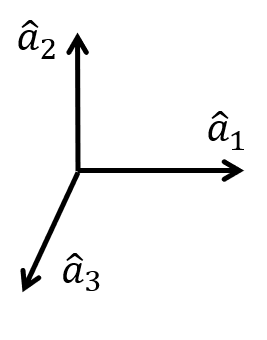
\includegraphics[width=0.20\textwidth]{base}
				\label{fig:base}}
				%%%%
				\hspace{10pt}
				%%%%
        \subfloat[Exemple]{
				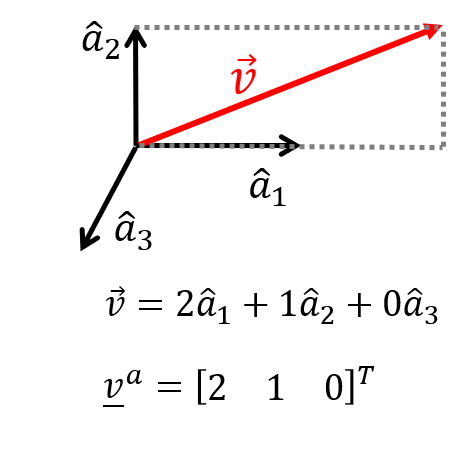
\includegraphics[width=0.25\textwidth]{baseex}
				\label{fig:baseex}}
				%%%%
				\hspace{10pt}
				%%%%
				\subfloat[Convention de la main droite]{
				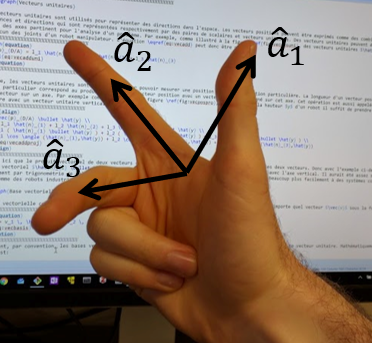
\includegraphics[width=0.25\textwidth]{righthand}
				\label{fig:righthand}}
        \caption{Les bases vectorielles}
				\label{fig:vecbasis}
\end{figure}
%%%%%%%%%%%%%%%%%%%%%%%%%%%%%%%%%%%%%%%%%%%%%%%%%%%%%%%%%%%%%%%%%

Mathématiquement, les critères de dimensions unitaires et d'orthogonalités sont donnés par les équations:
%%%%%%%%%%%%%%%%%%%%%%%%%%%%%%%%%%%
\begin{align}
\hat{a}_{1} \bullet \hat{a}_{1} = 1 \quad\quad \hat{a}_{2} \bullet \hat{a}_{2} = 1 \quad\quad \hat{a}_{3} \bullet \hat{a}_{3} = 1 
\label{eq:unit} \\
\hat{a}_{1} \bullet \hat{a}_{2} = 0 \quad\quad \hat{a}_{2} \bullet \hat{a}_{3} = 0 \quad\quad \hat{a}_{3} \bullet \hat{a}_{1} = 0
\label{eq:ortho}
\end{align} 
%%%%%%%%%%%%%%%%%%%%%%%%%%%%%%%%%%%
Normalement, par convention, les bases vectorielles suivent la règle de main droite (voir figure \ref{fig:righthand}) pour spécifier la direction du troisième vecteur unitaire. La convention de la main droite permet aussi de spécifier des relations en termes de produits vectoriels entre les vecteurs unitaires:
%%%%%%%%%%%%%%%%%%%%%%%%%%%%%%%%%%%
\begin{align}
\hat{a}_{1} = \hat{a}_{2} \times \hat{a}_{3} \quad\quad \hat{a}_{2} = \hat{a}_{3} \times \hat{a}_{1} \quad\quad \hat{a}_{3} = \hat{a}_{1} \times \hat{a}_{2} 
\label{eq:righthand}
\end{align} 
%%%%%%%%%%%%%%%%%%%%%%%%%%%%%%%%%%%

Les bases vectorielles permettent de faire des opérations et combiner des vecteurs en les exprimant avec une base commune de vecteurs unitaires. Dans la littérature, la notation $(\hat{i},\hat{j},\hat{k})$ ou $(\hat{x},\hat{y},\hat{z})$ est parfois utilisée. Dans ces notes, on utilisera des lettres ($a$,$b$,$c$,...) pour identifier des bases, ainsi que des indices (1,2,3) pour spécifier les trois axes (voir figure \ref{fig:base}). 
 

%%%%%%%%%%%%%%%%%%%%%%%%%%%%%%%%%%%%%%%%%%%%%%%
\subsection{Relation entre un vecteur et ses composantes dans une base}

Comme illustré à la figure \ref{fig:vecpospro2}, il est possible de calculer les composantes d'un vecteur exprimé dans une base par un produit scalaire du vecteur géométrique avec chacun des vecteurs unitaires de la base:
%%%%%%%%%%%%%%%%%%%%%%%%%%%%%%%%%%%
\begin{equation}
v_i^a = \vec{v} \bullet \hat{a}_i  \quad \Rightarrow \quad 
\col{v}^{a} = \left[ \begin{array}{c} \vec{v} \bullet \hat{a}_1 \\ \vec{v} \bullet \hat{a}_2 \\ \vec{v} \bullet \hat{a}_3  \end{array} \right] 
\end{equation} 
Inversement, comme illustré à la figure \ref{fig:vecpospro3}, le vecteur position géométrique peut être reconstruit en effectuant la somme des composantes multipliées avec leurs vecteurs unitaires respectifs:
%%%%%%%%%%%%%%%%%%%%%%%%%%%%%%%%%%%
\begin{equation}
\vec{v} = \sum_{i} v_i^a \hat{a}_i = v_1^a \hat{a}_1 + v_2^a \hat{a}_2 + v_3^a \hat{a}_3%= \left[ \begin{array}{c c c} p_1^a & p_2^a & p_3^a  \end{array} \right]  \left[ \begin{array}{c} \hat{a}_1 \\ \hat{a}_2 \\ \hat{a}_3  \end{array} \right] 
\end{equation} 
%%%%%%%%%%%%%%%%%%%%%%%%%%%%%%%%%%%
%%%%%%%%%%%%%%%%%%%%%%%%%%%%%%%%%%%%%%%%%%%%%%%%%%%%%%%%%%%%%%%
\begin{figure}[H]
				%\vspace{-10pt}
        \centering
        \subfloat[Projection sur une base vectorielle]{
				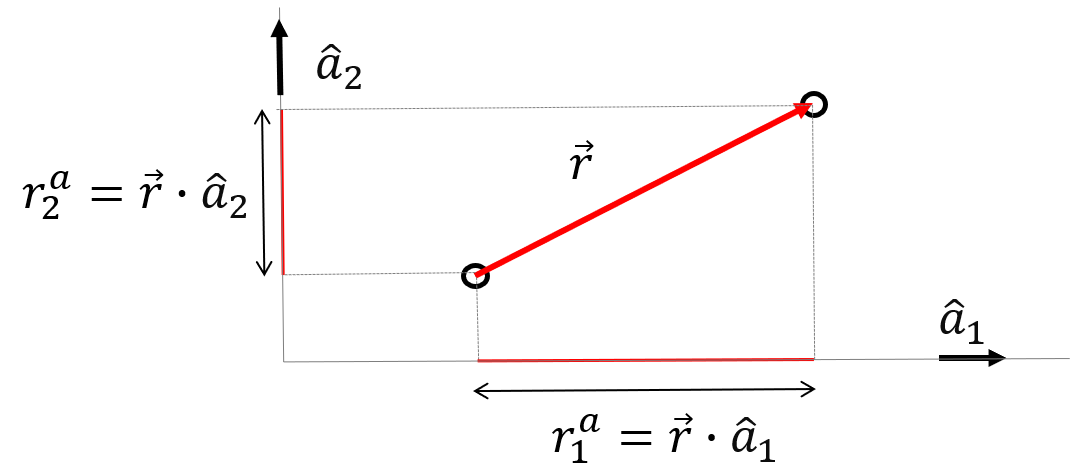
\includegraphics[width=0.50\textwidth]{vecpospro2.png}
				\label{fig:vecpospro2}}
				\hspace{+20pt}
				\subfloat[Décomposition selon les directions de la base]{
				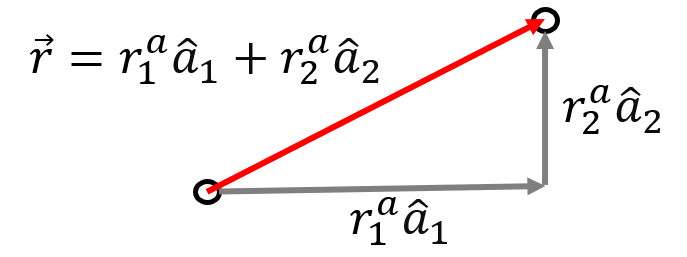
\includegraphics[width=0.40\textwidth]{vecpospro3.png}
				\label{fig:vecpospro3}}
				%\vspace{+30pt}
        \caption{Relations entre le vecteur géométrique de position et les composantes du vecteur-colonne}
				\label{fig:vecpospro23}
\end{figure}
%%%%%%%%%%%%%%%%%%%%%%%%%%%%%%%%%%%%%%%%%%%%%%%%%%%%%%%%%%%%%%%%%


%%%%%%%%%%%%%%%%%%%%%%%%%%%%%%%%%%%%%%%%%%%%%%%%%%%
\subsection{Transfert d'une équation vectorielle vers une équation matricielle} 
%
Lorsque les composantes de plusieurs vecteurs sont exprimées avec la même base, il est possible de faire des opérations directement avec les vecteur-colonnes de composantes. Cela permet de traiter simultanément les calculs de plusieurs axes, et aussi de faire des calculs numériques efficaces en utilisant les outils de l'algèbre linéaire. Par exemple, les additions et soustractions de vecteurs géométriques peuvent être calculées directement en termes des vecteur-colonnes dans une base:
%%%%%%%%%%%%%%%%%%%%%%%%%%%%%%%%%%%
\begin{equation}
\vec{u}   = \vec{v} + \vec{w}   \quad \Rightarrow \quad
\col{u}^a = \col{v}^a + \col{w}^a
\end{equation} 
%%%%%%%%%%%%%%%%%%%%%%%%%%%%%%%%%%%
Ce transfert d'une seule équation vectorielle à une équation matricielle (équivalent à un système de trois équations scalaires) correspond à une projection de l'équation vectorielle sur chacun des axes de la base:
%%%%%%%%%%%%%%%%%%%%%%%%%%%%%%%%%%%
\begin{equation}
\vec{u}   = \vec{v} + \vec{w}   
\quad \Rightarrow \quad
\left[ \begin{array}{c} (\vec{u}   = \vec{v} + \vec{w}  ) \bullet \hat{a}_1 \\ (\vec{u}   = \vec{v} + \vec{w}  ) \bullet \hat{a}_2 \\ (\vec{u}   = \vec{v} + \vec{w}  ) \bullet \hat{a}_3  \end{array} \right] 
\quad \Rightarrow \quad
\left[ \begin{array}{c}  u_1^a   = v_1^a + w_1^a   \\  u_2^a   = v_2^a + w_2^a   \\ u_3^a   = v_3^a + w_3^a   \end{array} \right] 
\quad \Rightarrow \quad
\col{u}^a = \col{v}^a + \col{w}^a
\end{equation} 
%%%%%%%%%%%%%%%%%%%%%%%%%%%%%%%%%%%

Les équations vectorielles avec des vecteurs de position peuvent donc être substituées par des équations matricielles équivalentes avec les vecteur-colonnes,\textbf{ à condition que tous les vecteur-colonnes soient exprimés dans une base commune}. 

%Voici quelques exemples de substitution d'équation de vecteurs de position vers des équations matricielles:
%%%%%%%%%%%%%%%%%%%%%%%%%%%%%%%%%%%%
%\begin{align}
%\vec{v}_{B/C}   = \vec{v}_{B/A} - \vec{v}_{C/A}   
%\quad &\Rightarrow \quad  \col{r}_{B/C}^a   = \col{r}_{B/A}^a - \col{r}_{C/A}^a 
%\\
%\vec{v}_{B/C}   = \vec{v}_{B/A} - \vec{v}_{C/A} \quad &\Rightarrow \quad \col{r}_{B/C}^b   = \col{r}_{B/A}^b - \col{r}_{C/A}^b 
%\\
%2  \vec{v}_{D/A} = 3 \vec{v}_{B/A} + \vec{v}_{C/A} \quad &\Rightarrow \quad  2  \col{r}_{D/A}^a = 3 \col{r}_{B/A}^a + \col{r}_{C/A}^a
%\end{align} 
%%%%%%%%%%%%%%%%%%%%%%%%%%%%%%%%%%%%





%%%%%%%%%%%%%%%%%%%%%%%%%%%%%%%%%%%%%%%%%%%%%%%%%%%
\section{Opérations vectorielles avec les vecteur-colonnes} 
\label{sec:opeveccol}
%
Les opérations vectorielles ont des équivalents en termes d'opérations matricielle avec les vecteur-colonnes qui sont très utiles pour les calculs numériques. Cette section introduit les opérations principales utiles pour la cinématique.

\subsection{Produit scalaire / produit intérieur}
Un produit scalaire peut être calculé directement par une opération matricielle avec les vecteur-colonnes appelée produit intérieur (\textit{inner product}):
%%%%%%%%%%%%%%%%%%%%%%%%%%%%%%%%%%%
\begin{equation}
\vec{u} \bullet \vec{v} = \col{u}^T \col{v} = \left[ \begin{array}{c c c} u_1 & u_2 & u_3  \end{array} \right]  \left[ \begin{array}{c} v_1 \\ v_2 \\ v_3  \end{array} \right]
= u_1 v_1 + u_2 v_2 + u_3 v_3
\end{equation} 
%%%%%%%%%%%%%%%%%%%%%%%%%%%%%%%%%%%
si $\col{u}$ et $\col{v}$ sont les composantes exprimées dans une base vectorielle commune, par exemple:
%%%%%%%%%%%%%%%%%%%%%%%%%%%%%%%%%%%
\begin{align}
\vec{u} \bullet \vec{v} &= (\col{u}^a)^T \col{v}^a = (\col{u}^b)^T \col{v}^b
\end{align} 
%%%%%%%%%%%%%%%%%%%%%%%%%%%%%%%%%%%
mais attention car: 
%%%%%%%%%%%%%%%%%%%%%%%%%%%%%%%%%%%
\begin{align}
\vec{u} \bullet \vec{v} &\ne (\col{u}^a)^T \col{v}^b \\
\vec{u} \bullet \vec{v} &\ne (\col{u}^b)^T \col{v}^a 
\end{align} 
%%%%%%%%%%%%%%%%%%%%%%%%%%%%%%%%%%%
Il est à noter que l'ordre de multiplication ne change pas le résultat pour le produit scalaire:
%%%%%%%%%%%%%%%%%%%%%%%%%%%%%%%%%%%
\begin{equation}
\vec{u} \bullet \vec{v} = \vec{v} \bullet \vec{u} = \col{u}^T \col{v} = \col{v}^T \col{u} 
\end{equation} 
%%%%%%%%%%%%%%%%%%%%%%%%%%%%%%%%%%%

%%%%%%%%%%%%%%%%%%%%%%%%%%%%%%%%%%%
\subsection{Produit vectoriel}
%
Un produit vectoriel (\textit{cross product}) peut être calculé directement par une opération matricielle définie avec les vecteur-colonnes:
%%%%%%%%%%%%%%%%%%%%%%%%%%%%%%%%%%%
\begin{equation}
\vec{u} = \vec{v} \times \vec{w} \quad \Rightarrow \quad  \col{u} = \col{v}^{\times}\col{w} \quad \Rightarrow \quad 
 \left[ \begin{array}{c} u_1 \\ u_2 \\ u_3  \end{array} \right] = 
\left[ \begin{array}{c c c}
	0 & -v_3 & v_2  \\ v_3 & 0 & -v_1 \\ -v_2 & v_1 & 0
\end{array}  \right]
 \left[ \begin{array}{c} w_1 \\ w_2 \\ w_3  \end{array} \right]
\end{equation} 
%%%%%%%%%%%%%%%%%%%%%%%%%%%%%%%%%%%
L'ordre de multiplication est important pour le produit vectoriel, il change la direction du vecteur résultant:
%%%%%%%%%%%%%%%%%%%%%%%%%%%%%%%%%%%
\begin{equation}
\vec{u} = \vec{v} \times \vec{w} =  -\vec{w} \times \vec{v} \quad \Rightarrow \quad  \col{u} = \col{v}^{\times}\col{w} = - \col{w}^{\times}\col{v}
\end{equation} 
%%%%%%%%%%%%%%%%%%%%%%%%%%%%%%%%%%%

\paragraph{Vecteurs unitaires d'une base vectorielle:}
Il est possible de calculer les composantes d'un vecteur unitaire qui complète une base vectorielle avec une opération de produit vectorielle, connaissant les composantes de deux vecteurs unitaires orthogonaux: 
%%%%%%%%%%%%%%%%%%%%%%%%%%%%%%%%%%%
\begin{equation}
\hat{b}_3 = \hat{b}_1 \times \hat{b}_2  \quad \Rightarrow \quad   \col{b}_3 = \col{b}_1^{\times}\col{b}_2
\end{equation} 
%%%%%%%%%%%%%%%%%%%%%%%%%%%%%%%%%%%

\paragraph{Note:}
Pour alléger la présentation, les exposants qui spécifient les bases vectorielles associées aux vecteur-colonnes sont parfois omis dans les équations, on considère alors que tous les vecteur-colonnes impliqués dans l'équation sont exprimés dans une base vectorielle commune.


%%%%%%%%%%%%%%%%%%%%%%%%%%%%%%%%%%%
\subsection{Produit tensoriel / produit extérieur}
%
Un produit tensoriel (\textit{outer-product}) peut être calculé directement par une opération matricielle définie avec les vecteur-colonnes:
%%%%%%%%%%%%%%%%%%%%%%%%%%%%%%%%%%%
\begin{equation}
\tensor{T} = \vec{v} \vec{w} \quad \Rightarrow \quad  T = \col{v} \, \col{w}^T = 
\left[ \begin{array}{c}     v_1 \\ v_2 \\ v_3  \end{array} \right]
\left[ \begin{array}{c c c} w_1 &  w_2 &  w_3  \end{array} \right] = 
\left[ \begin{array}{c c c}
v_1 w_1 & v_1 w_2 & v_1 w_3  \\ 
v_2 w_1 & v_2 w_2 & v_2 w_3         \\ 
v_3 w_1 & v_3 w_2 & v_3 w_3 
\end{array}  \right]
\end{equation} 
%%%%%%%%%%%%%%%%%%%%%%%%%%%%%%%%%%%
où le matrice $T$ correspond aux composantes du tenseur $\tensor{T}$, avec comme correspondance si toutes les composantes sont relatives à une base $a$ :
%%%%%%%%%%%%%%%%%%%%%%%%%%%%%%%%%%%
\begin{equation}
\tensor{T} = T_{11} \hat{a}_1 \hat{a}_1  + T_{12} \hat{a}_1 \hat{a}_2 + \hdots + T_{23} \hat{a}_2 \hat{a}_3  + T_{33} \hat{a}_3 \hat{a}_3 
\end{equation} 
%%%%%%%%%%%%%%%%%%%%%%%%%%%%%%%%%%%

%%%%%%%%%%%%%%%%%%%%%%%%%%%%%%%%%%%
\subsection{Changement de base}
%
Les composantes d'un vecteur géométrique $\vec{v}$ dans une base $a$ peuvent être directement reliées aux composantes du même vecteur géométrique $\vec{v}$ dans une autre base $b$, par une équation matricielle qui implique les vecteur-colonnes et une matrice 3$\times$3 appelée une \textit{matrice de rotation}. On va noter une matrice $^bR^a$ lorsqu'une multiplication par la gauche de cette matrice avec un vecteur colonne $\col{v}^a$ donne le vecteur-colonne $\col{v}^b$:
%%%%%%%%%%%%%%%%
\begin{align}
\col{v}^b &= {}^bR^a \col{v}^a  \quad \Rightarrow \quad
 \left[ \begin{array}{c} v_1^b \\ v_2^b \\ v_3^b  \end{array} \right]
=
\left[ \begin{array}{c c c}
	{}^bR^a_{11} & {}^bR^a_{12} & {}^bR^a_{13} \\ 
	{}^bR^a_{21} & {}^bR^a_{22} & {}^bR^a_{23} \\
	{}^bR^a_{31} & {}^bR^a_{32} & {}^bR^a_{33}
\end{array}  \right]
 \left[ \begin{array}{c} v_1^a \\ v_2^a \\ v_3^a  \end{array} \right]
\label{eq:basechange1}
\end{align} 
%%%%%%%%%%%%%%%%%
Les propriétés et le calcul des matrices de rotation seront traités en détails à la section \ref{sec:changematrice}.



%%%%%%%%%%%%%%%%%%%%%%%%%%%%%%%%%%%%%%%%%%%%%%%%%%%%
%\subsection{Calculs appliqués dans un contexte de cinématique} 
%%
%\paragraph{Normes, projections et calcul d'angles:}
%Lorsque qu'on connait les composantes de vecteurs dans une base commune, le produit intérieur peut être utilisé pour calculer la longueur d'un vecteur position:
%%%%%%%%%%%%%%%%%%%%%%%%%%%%%%%%%%%%
%\begin{align}
%\|\vec{r}\|^2 &= \vec{r} \bullet \vec{r} = \col{r}^T \col{r} = r_1^2 + r_2^2 + r_3^2
%\end{align} 
%%%%%%%%%%%%%%%%%%%%%%%%%%%%%%%%%%%%
%pour calculer une distance projeté selon un axe décrit par un vecteur unitaire $\hat{n}$:
%%%%%%%%%%%%%%%%%%%%%%%%%%%%%%%%%%%%
%\begin{align}
%d_n &= \vec{r} \bullet \hat{n} = \col{r}^T \col{n} = r_1 n_1 + r_2 n_2 + r_3 n_3
%\end{align} 
%%%%%%%%%%%%%%%%%%%%%%%%%%%%%%%%%%%%
%et pour calculer un angle entre deux vecteurs unitaires $\hat{x}$ et $\hat{y}$:
%%%%%%%%%%%%%%%%%%%%%%%%%%%%%%%%%%%%
%\begin{align}
%\cos \angle (\hat{x},\hat{y}) = \hat{x} \bullet \hat{y} = \col{x}^T \col{y} = x_1 y_1 + x_2 y_2 + x_3 y_3
%\end{align} 
%%%%%%%%%%%%%%%%%%%%%%%%%%%%%%%%%%%%
%
%\paragraph{Vecteurs unitaires:}
%Il est possible de calculer les composantes d'un vecteur unitaire qui complète une base vectorielle avec une opération de produit vectorielle, connaissant les composantes de deux vecteurs unitaires orthogonaux: 
%%%%%%%%%%%%%%%%%%%%%%%%%%%%%%%%%%%%
%\begin{equation}
%\hat{b}_3 = \hat{b}_1 \times \hat{b}_2  \quad \Rightarrow \quad   \col{b}_3 = \col{b}_1^{\times}\col{b}_2
%\end{equation} 
%%%%%%%%%%%%%%%%%%%%%%%%%%%%%%%%%%%%


%%%%%%%%%%%%%%%%%%%%%%%%%%%%%%%%%%%%%%%%%%%%%%%%%%%
\subsection{Invariants} 
%
Le vecteur géométrique $\vec{v}$ est une quantité constante peu importe la base vectorielle utilisée: 
%%%%%%%%%%%%%%%
\begin{equation}
\vec{v} = \sum_{i} v_i^a \hat{a}_i = \sum_{i} v_i^b \hat{b}_i = \sum_{i} v_i^c \hat{c}_i
\end{equation}
%%%%%%%%%%%%%%%
mais le vecteur-colonne dépend de la base vectorielle. Les vecteur-colonnes sont en générale différents sauf dans le cas particulier de bases vectorielles coïncidentes:
%%%%%%%%%%%%%%%%%%%%%%%%%%%%%%%%%%%
\begin{equation}
\col{v}^{a} \ne \col{v}^{b} \quad\quad \text{sauf dans le cas particulier:} \quad \hat{a}_1 = \hat{b}_1 \;,\; \hat{a}_2 = \hat{b}_2  \;\text{et}\; \hat{a}_3 = \hat{b}_3 
\end{equation} 
%%%%%%%%%%%%%%%%%%%%%%%%%%%%%%%%%%%
La longueur du vecteur-géométrique étant une constante peut importe la base vectorielle utilisée, il est possible d'établir la relation suivante entre les vecteur-colonnes utilisant différentes bases:
%%%%%%%%%%%%%%%
\begin{equation}
\|\vec{v}\|^2 = \vec{v} \bullet \vec{v} = (\col{v}^{a})^T \col{v}^{a} = (\col{v}^{b})^T \col{v}^{b} = (\col{v}^{c})^T \col{v}^{c}
\end{equation}
%%%%%%%%%%%%%%%
La norme des vecteur-colonnes est donc invariante par rapport au choix de la base. 






 %%%%%%%%%%%%%%%%%%%%%%%%%%%%%%%%%%%%%%%%%%%%%%%%%%%%%%%%%%%%%%%%%%%%
\newpage
\section{Summary of vector operations in terms of components}

\begin{table}[H]
%\caption{ Basic Vectorial Operations }
\label{basic}
 \begin{tabular}{ | c | c | c |}
 \hline
 Vector and Tensors & Matrix, Row and Columns & Components and index \\
 %%%%%%%%%%%%%%%%%%%%%%%%%%%%%%%%%%%%%%%%%%%%%%%%%%%%%%%%%%%%%%%%%%%%
 \hline
 \multicolumn{3}{| c |}{Definitions} \\
 \hline
 %%%%%%%%%%%%%%%%%%%%%%%%%%%%%%%%%%%%%%%%%%%%%%%%%%%%%%%%%%%%%%%%%%%%
 Vector $\vec{v}$ and Tensor $\vec{\vec{T}}$ 
 &
 Column $\underline{c}$, Row $\underline{r}$ and Matrix $M$ 
 &
 Scalar components $x_i$ and  $x_{ij}$ 
 \\ & & \\
 %%%%%%%%%%%%%%%%%%%%%%%%%%%%%%%%%%%%%%%%%%%%%%%%%%%%%%
 %  1-D
 %%%%%%%%%%%%%%%%%%%%%%%%%%%%%%%%%%%%%%%%%%%%%%%%%%%%%%
 $\vec{v} = x_1 \vec{i} + x_2 \vec{j} + x_3 \vec{k}$ 
 &
 $\underline{c} = \left[ \begin{array}{c} x_1 \\ x_2 \\x_3 \end{array} \right] $
 $\underline{r} = \left[ \begin{array}{c c c } x_1 & x_2 & x_3 \end{array} \right] $
 &
 $x_i \quad i \in \{ 1,2,3\}$
 \\ && \\
 %%%%%%%%%%%%%%%%%%%%%%%%%%%%%%%%%%%%%%%%%%%%%%%%%%%%%%
 %  2-D
 %%%%%%%%%%%%%%%%%%%%%%%%%%%%%%%%%%%%%%%%%%%%%%%%%%%%%%
 $\vec{\vec{T}} = x_{11} \vec{i}\vec{i} +  x_{12} \vec{i}\vec{j} + ... + x_{33}  \vec{k}\vec{k}$
 &
 $ M = \left[ \begin{array}{c c c } 
 x_{11} & x_{12} & x_{13} \\  
 x_{21} & x_{22} & x_{23} \\  
 x_{31} & x_{32} & x_{33} \\  
 \end{array} \right] $
 &
 $x_{ij} \quad i \in \{ 1,2,3\} \; j \in \{ 1,2,3\}$
 \\ && \\
 %%%%%%%%%%%%%%%%%%%%%%%%%%%%%%%%%%%%%%%%%%%%%%%%%%%%%%%%%%%%%%%%%%%%
 \hline 
 \multicolumn{3}{| c |}{Dot or inner product} \\
 \hline && \\
 %%%%%%%%%%%%%%%%%%%%%%%%%%%%%%%%%%%%%%%%%%%%%%%%%%%%%%%%%%%%%%%%%%%%
 $z = \vec{x} \bullet \vec{y}$ 
 &
 $z = \underline{x}^T \underline{y} = \left[ \begin{array}{c c c } x_1 & x_2 & x_3 \end{array} \right] \left[ \begin{array}{c} y_1 \\ y_2 \\ y_3 \end{array} \right] $
 &
 $z = \sum_{ij}{ x_i y_j \delta_{ij}} = \sum_{i}{x_i y_i} $
 \\ && \\
 $\vec{z} = \vec{\vec{A}} \bullet \vec{x}$ 
 &
 $\underline{z}  = A \underline{x} = \left[ \begin{array}{c c c } 
 a_{11} & a_{12} & a_{13} \\
 a_{21} & a_{22} & a_{23} \\
 a_{31} & a_{32} & a_{33} 
 \end{array} \right] \left[ \begin{array}{c} x_1 \\ x_2 \\ x_3 \end{array} \right] $
 &
 $z_i = \sum_{jk}{ a_{ij} x_k \delta_{jk}} = \sum_{j}{a_{ij} x_j} $
 \\ && \\
 $\vec{z} = \vec{x} \bullet \vec{\vec{A}}$ 
 &
 $\underline{z}  = \underline{x}^T A $
 &
 $z_j = \sum_{ik}{ x_k a_{ij} \delta_{ki}} = \sum_{i}{x_i a_{ij}} $
 \\ && \\
 %%%%%%%%%%%%%%%%%%%%%%%%%%%%%%%%%%%%%%%%%%%%%%%%%%%%%%%%%%%%%%%%%%%%
 \hline
 \multicolumn{3}{| c |}{Dyadic or outer product} \\
 \hline && \\
 %%%%%%%%%%%%%%%%%%%%%%%%%%%%%%%%%%%%%%%%%%%%%%%%%%%%%%%%%%%%%%%%%%%%
 $\vec{\vec{Z}} = \vec{x}  \vec{y}$ 
 &
 $Z = \underline{x} \, \underline{y}^T = \left[ \begin{array}{c } x_1 \\ x_2 \\ x_3 \end{array} \right] \left[ \begin{array}{c c c} y_1 & y_2 & y_3 \end{array} \right] $
 &
 $z_{ij} = x_i \, y_j $
 \\ && \\
 %%%%%%%%%%%%%%%%%%%%%%%%%%%%%%%%%%%%%%%%%%%%%%%%%%%%%%%%%%%%%%%%%%%%
 \hline
 \multicolumn{3}{| c |}{Cross product} \\
 \hline && \\
 %%%%%%%%%%%%%%%%%%%%%%%%%%%%%%%%%%%%%%%%%%%%%%%%%%%%%%%%%%%%%%%%%%%%
 $\vec{z} = \vec{x} \times \vec{y}$ 
 &
 $\underline{z} = \underline{x}^{\times} \underline{y} = \left[ \begin{array}{c c c } 
  0   & -x_3 & x_2 \\
  x_3 & 0    & -x_1 \\
 -x_2 & x_1  & 0 
 \end{array} \right] \left[ \begin{array}{c} y_1 \\ y_2 \\ y_3 \end{array} \right] $
 &
 $z_i = \sum_{jk}{ \epsilon_{ijk} x_j y_k } $
 \\ && \\
\hline
 \end{tabular}
\end{table}

\subsection{Index notation special symbols}

\subsubsection{ Kronecker delta }
\begin{align}
\delta_{ij} = \left\lbrace \begin{array}{c}
1 \quad\text{if}\quad i=j\\
0 \quad\text{if}\quad i\neq j
\end{array}
\right.
\end{align}


\subsubsection{ Levi-Civita permutation symbol }
\begin{align}
\epsilon_{ijk} = \left\lbrace \begin{array}{l}
+1  \quad\text{if}\quad ijk=(123),(231) \;\text{or}\; (312)\\
-1   \quad\text{if}\quad ijk=(321),(213) \;\text{or}\; (132)\\
\,0  \quad\text{if an index is repeated}
\end{array}
\right.
\end{align}



\section{Column-vector and matrix differentiation}
\label{sec:vecmatdifferentiation}

Note that the shape of vector/matrix resulting from a multi-axis differentiation is a question of layout convention. The numerator layout convention is used here. Identities presented need to be transposed if using a denominator layout instead. There is no ambiguity with the index representation.

\subsubsection{Scalar by Scalar}

For a scalar function $y = f(x)$: 
%%%%%%%%%%%%%%%%%%%%%%%%
\begin{align}
%y = f(x) \quad \quad 
z = \frac{\partial y}{\partial x}
\end{align}
%%%%%%%%%%%%%%%%%%%%%


\subsubsection{Vector by Scalar}

For the derivation of a vector function $\underline{y} = f(x)$ where $\underline{y} \in \mathbb{R}^n$ with respect to a scalar $x$, by convention if the numerator $\underline{y}$ is a $n \times 1$ column vector, the result is a $n \times 1$ column vector too:
%%%%%%%%%%%%%%%%%%%%%%%%%%%
\begin{align}
\underline{z} = \frac{\partial \underline{y}}{\partial x} =  
 \left[ \begin{array}{c } 
  \frac{\partial y_1}{\partial x}   \\ \vdots \\ \frac{\partial y_n}{\partial x}
 \end{array} \right]
 \quad\Leftrightarrow\quad
 z_{i} = \frac{\partial y_i}{\partial x}
\end{align}
%%%%%%%%%%%%%%%%%%%%%%%%%%%


\subsubsection{Scalar by Vector}

For the gradient of a multi-inputs scalar function $y = f(\underline{x})$ where $\underline{x} \in \mathbb{R}^n$, by convention if the denominator $\underline{x}$ is a $n \times 1$ column vector, the result is a $1 \times n$ row vector:
%%%%%%%%%%%%%%%%
\begin{align}
\underline{z} = \frac{\partial y}{\partial \underline{x}} &= 
 \left[ \begin{array}{c c c } 
  \frac{\partial y}{\partial x_1}   & ... & \frac{\partial y}{\partial x_n}
 \end{array} \right]
 \quad \Leftrightarrow\quad
 z_i = \frac{\partial y}{\partial x_i}
\end{align}
%%%%%%%%%%%%%%%%%%%
%\begin{align}
%\frac{\partial y}{\partial \underline{x}^T} &= \underline{z}^T = 
%\left[ \begin{array}{c } 
%  \frac{\partial y}{\partial x_1}   \\ \vdots \\ \frac{\partial y}{\partial x_n}
% \end{array} \right]
% & \quad \Leftrightarrow\quad
% z_j = \frac{\partial y}{\partial x_j}
%\end{align}

\begin{table}[H]
\centering
\caption{ Scalar by a vector: Identities}
\label{scavec}
 \begin{tabular}{ | c | c | c |}
 \hline \hline & & \\
 Scalar $y = f(\underline{x})$ expression & Gradient Vector $\frac{\partial y}{\partial \underline{x}}$  & Notes \\ & & \\
 \hline \hline & & \\
 $ \underline{a}^T \underline{x} = \underline{x}^T \underline{a} $ & 
 $\underline{a}^T$ &   If $\underline{a}$ is not a function of $\underline{x}$
 \\ & & \\
  \hline & & \\
 $ \underline{x}^T \underline{x} $ & 
 $ 2 \, \underline{x}^T $ &   
 \\ & & \\
 \hline & & \\
 $ \underline{x}^T A \underline{x} $ & 
 $\underline{x}^T ( A + A^T )$ &   If $A$ is not a function of $\underline{x}$
 \\ & & \\
 \hline & & \\
 $ \underline{x}^T A \underline{x} $ & 
 $ 2\, \underline{x}^T A$ &   If $A$ is symmetric and not a function of $\underline{x}$
 \\ & & \\
 \hline
 \end{tabular}
\end{table}

\subsubsection{Vector by Vector}
For the gradient of a multi-inputs vector function $\underline{y} = f(\underline{x})$ where $\underline{x} \in \mathbb{R}^n$ and $\underline{y} \in \mathbb{R}^m$, by convention if the numerator $\underline{y}$ is a $m \times 1$ column vector and the denominator a $n \times 1$ column vector, the result is a $m \times n$ matrix, often called the Jacobian matrix:

%%%%%%%%%%%%%%%%%%%%%%%%%%%%%%%
\begin{align}
Z = \frac{\partial \underline{y}}{\partial \underline{x}} =  
\left[ \begin{array}{c c c } 
  \frac{\partial y_1}{\partial x_{1}}   & ... & \frac{\partial y_1}{\partial x_{n}} \\
  \vdots                             & ... & \vdots                          \\
  \frac{\partial y_m}{\partial x_{1}}   & ... & \frac{\partial y_m}{\partial x_{n}} \\
 \end{array} \right]
 \quad\Leftrightarrow\quad
  z_{ij} = \frac{\partial y_i}{\partial x_j}
\end{align}
%%%%%%%%%%%%%%%%%%%%%%%%%%%%%

\begin{table}[H]
\centering
\caption{ Vector by a vector: Identities}
\label{scavec}
 \begin{tabular}{ | c | c | c |}
 \hline \hline & & \\
 Vector $\underline{y} = f(\underline{x})$ expression &Jacobian Matrix $\frac{\partial \underline{y}}{\partial \underline{x}}$  & Notes \\ & & \\
 \hline \hline & & \\
 $ \underline{x} $ & 
 $I$ &   Identity Matrix
 \\ & & \\
 \hline & & \\
 $ A \underline{x} $ & 
 $A$ &   If $A$ is not a function of $\underline{x}$
 \\ & & \\
 \hline & & \\
 $ \underline{x}^T A $ & 
 $A^T$ &   If $A$ is not a function of $\underline{x}$
 \\ & & \\
 \hline
 \end{tabular}
\end{table}

%\subsubsection{Vector by Matrix}
%3rd order tensor..

\subsubsection{Matrix by Scalar}

For the gradient of a matrix function $\underline{A} = f(x)$ where $x$ is a scalar and $A$ is a $n \times m$ matrix, the result is also a $n \times m$ matrix:
%%%%%%%%%%%%%%%%%%%%%%%%%%%%
\begin{align}
Z = \frac{\partial A}{\partial x} =  
\left[ \begin{array}{c c c } 
  \frac{\partial a_{11}}{\partial x}   & ... & \frac{\partial a_{1m}}{\partial x} \\
  \vdots                             & ... & \vdots                          \\
  \frac{\partial a_{n1}}{\partial x}   & ... & \frac{\partial a_{nm}}{\partial x} \\
 \end{array} \right]
 \quad\Leftrightarrow\quad
  z_{ij} = \frac{\partial a_{ij}}{\partial x}
\end{align}
%%%%%%%%%%%%%%%%%%%%%%%%%%%

\begin{table}[H]
\centering
\caption{ Matrix by scalar: Identities}
\label{scavec}
 \begin{tabular}{ | c | c | c |}
 \hline \hline & & \\
 Matrix $A$ expression & Differential Matrix $\frac{\partial A}{\partial x}$  & Notes \\ & & \\
 \hline \hline & & \\
 $ M^{-1} $ & 
 $ -M^{-1} \frac{\partial M}{\partial x} M^{-1} $ &   
 \\ & & \\
 \hline
 \end{tabular}
\end{table}



\subsubsection{Scalar by Matrix}

For the gradient of a multi-inputs scalar function $y = f( A )$ where $A$ is an $n \times m$ matrix, by convention the result is a $m \times n$ matrix:
%%%%%%%%%%%%%%%%%%%%%%%%%%%%%%%%%%%%
\begin{align}
Z = \frac{\partial y}{\partial A} =  
\left[ \begin{array}{c c c } 
  \frac{\partial y}{\partial a_{11}}   & ... & \frac{\partial y}{\partial a_{1n}} \\
  \vdots                             & ... & \vdots                          \\
  \frac{\partial y}{\partial a_{m1}}   & ... & \frac{\partial y}{\partial a_{mn}} \\
 \end{array} \right]
 \quad\Leftrightarrow\quad
 z_{ji} = \frac{\partial y}{\partial a_{ij}}
\end{align}
%%%%%%%%%%%%%%%%%%%%%%%%%%%%%%%%%%%

\begin{table}[H]
\centering
\caption{ Scalar by Matrix: Identities}
\label{scavec}
 \begin{tabular}{ | c | c | c |}
 \hline \hline & & \\
 Scalar $y$ expression & Differential Matrix $\frac{\partial y}{\partial A}$  & Notes \\ & & \\
 \hline \hline & & \\
 $ \underline{a}^T A \, \underline{b} $ & 
 $ \underline{b} \, \underline{a}^T   $ &    $\underline{a}$ and  $\underline{b}$ are not function of $A$
 \\ & & \\
 $ \underline{a}^T A^T A \, \underline{b} $ & 
 $ \underline{a} \, \underline{b}^T A^T + \underline{b} \, \underline{a}^T  A^T  $ &    $\underline{a}$ and  $\underline{b}$ are not function of $A$
 \\ & & \\
 \hline
 \end{tabular}
\end{table}

%Note that while the numerator layout is generally preferred, the denominator layout is used for scalar by matrix differentiation, because more natural in this situation. However, this would be conflicting with the typical gradient layout when $m=1$.

%\subsubsection{Matrix by Vector}
%3rd order tensor..

%\subsubsection{Matrix by Matrix}
%4rd order tensor..

\newpage

\subsection{Examples}

\subsubsection{Gradient of Quadratic Function}

Finding the gradient $\frac{\partial f}{\partial \underline{x}}$ of the quadratic function $f=\underline{x}^T A \underline{x}$. First converting to index notations:
\begin{align}
f = \sum_{ij}{x_i A_{ij} x_j}
\end{align}
Then differentiating per $x_k$ components:
\begin{align}
\frac{\partial f}{\partial x_k} &= \sum_{ij}{  \frac{\partial}{\partial x_k} \left(x_i A_{ij} x_j \right)} \\
\frac{\partial f}{\partial x_k} &= \sum_{ij}{\left( \underbrace{ \frac{\partial x_i}{\partial x_k}}_{\delta_{ik}}  A_{ij} x_j + x_i \underbrace{\frac{\partial A_{ij} }{\partial x_k}}_{0} x_j + x_i A_{ij} \underbrace{\frac{\partial x_j}{\partial x_k}}_{\delta_{jk}} \right)} \\
\frac{\partial f}{\partial x_k} &= \sum_{ij}{  \delta_{ik}  A_{ij} x_j } + \sum_{ij}{  \delta_{jk} x_i A_{ij} }\\
\frac{\partial f}{\partial x_k} &= \sum_{j}{  A_{kj} x_j } + \sum_{i}{ x_i A_{ik} }\\
\frac{\partial f}{\partial x_k} &= \sum_{i}{\left(  A_{ki} x_i  + x_i A_{ik} \right)}\\
%\frac{\partial f}{\partial x_k} &= \sum_{i}{ x_i \left(  A_{ik} + A_{ki} \right)  }\\
\end{align}
Which correspond in matrix form, with the numerator layout convention, to:
\begin{align}
\frac{\partial f}{\partial \underline{x}} = \underline{x}^T ( A + A^T )
\end{align}

\subsubsection{Least square solution derivation in vector form}

Minimizing the error norm $\|\underline{e}\|^2$ of the estimation problem $\underline{e} = A \underline{\hat{x}} - \underline{b}$ by selecting the parameters $\underline{\hat{x}}$. If the gradient of the error norm with respect to the parameter vector is set to zero:
\begin{align}
\underline{0} &= \frac{\partial \|\underline{e}\|^2 }{\partial \underline{\hat{x}}} = \frac{\partial (\underline{e}^T \underline{e} )}{\partial \underline{\hat{x}}} = 2 \, \underline{e}^T \frac{\partial \underline{e} }{\partial \underline{\hat{x}}} = 2\, (A \underline{\hat{x}} - \underline{b})^T A 
\end{align}
For which the solution is
\begin{align}
\underline{\hat{x}} = \left[ A^T A \right]^{-1} A^T \underline{b}
\end{align}